\section{Open questions}
\subsection{A refinement of GTKP}
The result we have spent the most time trying to obtain is the following refinement:
\begin{conjecture}
    A class of compact polyhedra is modally definable if and only if
    it is closed under finite disjoint unions and simplicial up-reductions.
\end{conjecture}

The procedure we have in mind to prove the equivalence between the current result
and the one above is the following:
\begin{itemize}
    \item Consider the face up-reduction $f:P\fupred Q$ realized as $f:P\upred [L]$;
    \item Realize $f$ as a map $\tilde{f}:[K]\upred [L]$;
    \item Construct an up-reduction $\tilde{g}:K\upred L$ ``informed by $\tilde{f}$''
    that is an up-reduction and a map of simplicial complexes;
    \item Realize $\tilde{g}$ as a simplicial up-reduction $g:P\upred Q$.
\end{itemize}
If $\tilde{f}$ were (or were densely contained in) a map of (abstract) simplicial complexes, rather than merely one of posets, our work would be done: it is possible to realize any map of ASCs as a simplicial map of their polyhedra.

In general, though, this is not the case. Consider $P$ to be three segments and $Q$ the triangle (the boundary of the $2$-simplex):

\begin{figure}[H]
  \centering
  \begin{tikzpicture}[scale=1]
  % Coordinates
  \coordinate (A) at (0.00, 0.00);
  \coordinate (B) at (2.00, 0.00);
  \coordinate (D) at (0.00, 1.00);
  \coordinate (E) at (2.00, 1.00);
  \coordinate (F) at (0.00, 2.00);
  \coordinate (J) at (4.00, 0.00);
  \coordinate (K) at (4.00, 2.00);
  \coordinate (L) at (5.50, 2.00);
  \coordinate (M) at (7.00, 0.00);
  \coordinate (N) at (7.00, 2.00);
  \coordinate (O) at (5.50, 0.00);
  \coordinate (P) at (4.00, 4.00);
  \coordinate (Q) at (7.00, 4.00);
  \coordinate (R) at (5.50, 6.50);
  \coordinate (G) at (2.00, 2.00);
  \coordinate (H) at (1.00, 2.00);
  \coordinate (I) at (1.00, 1.00);
  \coordinate (C) at (1.00, 0.00);

  % Drawing
  \draw (A) -- (B);
  \draw (D) -- (E);
  \draw (F) -- (G);
  \draw (J) -- (K);
  \draw (J) -- (L);
  \draw (L) -- (M);
  \draw (M) -- (N);
  \draw (K) -- (O);
  \draw (O) -- (N);
  \draw[gray] (P) -- (Q) -- (R) -- cycle;
  \draw[pastelred, thick] (F) -- node[above, text=pastelred, midway] {$ac$} (H);
  \draw (H) -- (G);
  \draw[pastelgreen, thick] (H) -- node[above, text=pastelgreen, midway] {$bc$} (G);
  \draw[pastelviolet, thick] (I) -- node[above, text=pastelviolet, midway] {$ab$} (E);
  \draw[pastelred, thick] (C) -- node[above, text=pastelred, midway] {$ac$} (B);
  \draw[pastelviolet, thick] (A) -- node[above, text=pastelviolet, midway] {$ab$} (C);
  \draw[pastelgreen, thick] (D) -- node[above, text=pastelgreen, midway] {$bc$} (I);
  \draw[pastelviolet,thick] (P) -- (Q);
  \draw[pastelred, thick] (P) -- (R);
  \fill[pastelred] (B) circle (1pt);
  \draw[pastelgreen, thick] (R) -- (Q);
  \fill[pastelviolet] (A) circle (1pt);
  \fill[pastelgreen] (D) circle (1pt);
  \fill[pastelviolet] (E) circle (1pt);
  \fill[pastelred] (F) circle (1pt);
  \fill[pastelblue] (J) circle (1pt);
  \node[above left, pastelblue] at (J) {$a$};
  \fill[pastelviolet] (K) circle (1pt);
  \node[above left, pastelviolet] at (K) {$ab$};
  \fill[pastelred] (L) circle (1pt);
  \node[above, pastelred] at (L) {$ac$};
  \fill[pastelblue] (M) circle (1pt);
  \node[above right, pastelblue] at (M) {$c$};
  \fill[pastelgreen] (N) circle (1pt);
  \node[above right, pastelgreen] at (N) {$bc$};
  \fill[pastelblue] (O) circle (1pt);
  \node[above, pastelblue] at (O) {$b$};
  \fill[pastelblue] (P) circle (1pt);
  \node[below left, pastelblue] at (P) {$a$};
  \fill[pastelblue] (Q) circle (1pt);
  \node[below right, pastelblue] at (Q) {$b$};
  \fill[pastelblue] (R) circle (1pt);
  \node[left, pastelblue] at (R) {$c$};
  \fill[pastelgreen] (G) circle (1pt);
  \fill[pastelblue] (H) circle (1pt);
  \node[above, pastelblue] at (H) {$c$};
  \fill[pastelblue] (I) circle (1pt);
  \node[above, pastelblue] at (I) {$b$};
  \fill[pastelblue] (C) circle (1pt);
  \node[above, pastelblue] at (C) {$a$};
  \fill[pastelblue] (J) circle (1pt);
  \node[above left, pastelblue] at (J) {$a$};
  \fill[pastelviolet] (K) circle (1pt);
  \node[above left, pastelviolet] at (K) {$ab$};
  \fill[pastelred] (L) circle (1pt);
  \node[above, pastelred] at (L) {$ac$};
  \fill[pastelblue] (M) circle (1pt);
  \node[above right, pastelblue] at (M) {$c$};
  \fill[pastelgreen] (N) circle (1pt);
  \node[above right, pastelgreen] at (N) {$bc$};
  \fill[pastelblue] (O) circle (1pt);
  \node[above, pastelblue] at (O) {$b$};
  \fill[pastelblue] (P) circle (1pt);
  \node[below left, pastelblue] at (P) {$a$};
  \fill[pastelblue] (Q) circle (1pt);
  \node[below right, pastelblue] at (Q) {$b$};
  \fill[pastelblue] (R) circle (1pt);
  \node[left, pastelblue] at (R) {$c$};
  \fill[pastelblue] (H) circle (1pt);
  \node[above, pastelblue] at (H) {$c$};
  \fill[pastelblue] (I) circle (1pt);
  \node[above, pastelblue] at (I) {$b$};
  \fill[pastelblue] (C) circle (1pt);
  \node[above, pastelblue] at (C) {$a$};
\end{tikzpicture}
\caption{An example of a face up-reduction that does not come from a simplicial up-reduction}
\end{figure}

The Hasse diagram (bottom right) is $L$; the three segments are $P$, and the triangle is $Q$. The map is indicated by the coloring.

One can check that it is a p-morphism, but clearly not a map of simplicial complexes, since the images of the vertices are not themselves vertices.

\subsection{The precompact case}

How do things change if we allow open polyhedra? We gain access to generated subframes, but the relationship between polyhedra and simplicial complexes becomes looser:

Consider the poset consisting of a single point: it is the poset of the maximal face of any simplex.

Moreover, even if we try to circumvent this problem by considering the closure of a face --- which is indeed a simplicial complex --- we can find cases where the combinatorial description fails to be PL-invariant.

For example, consider the disjoint union of two triangles:
\begin{figure}[H]
  \centering
  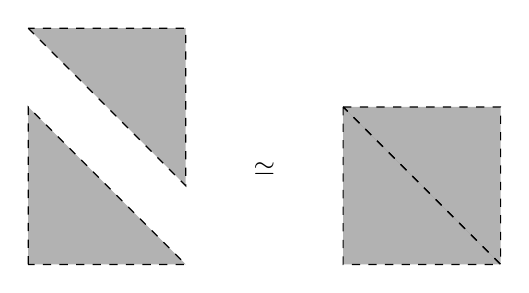
\begin{tikzpicture}[scale=1]
  % Coordinates
  \coordinate (A) at (0.00, 0.00);
  \coordinate (B) at (0.00, 2.00);
  \coordinate (C) at (2.00, 0.00);
  \coordinate (D) at (0.00, 3.00);
  \coordinate (E) at (2.00, 1.00);
  \coordinate (F) at (2.00, 3.00);
  \coordinate (G) at (3.00, 1.01);
  \coordinate (H) at (4.00, 2.00);
  \coordinate (I) at (4.00, 0.00);
  \coordinate (J) at (6.00, 0.00);
  \coordinate (K) at (6.00, 2.00);

  % Drawing
  \filldraw[dashed, fill=black, fill opacity=0.3] (A) -- (B) -- (C) -- cycle;
  \filldraw[dashed, fill=black, fill opacity=0.3] (D) -- (E) -- (F) -- cycle;
  \filldraw[dashed, fill=black, fill opacity=0.3] (H) -- (I) -- (J) -- cycle;
  \filldraw[dashed, fill=black, fill opacity=0.3] (H) -- (K) -- (J) -- cycle;
  \node[above, black] at (G) {$\simeq$};
\end{tikzpicture}
\end{figure}

The two objects are PL-homeomorphic, but their simplicial complexes are not.
\subsection{The infinite case}

An interesting question is what happens when we allow arbitrarily large simplicial complexes, both in dimension and in number of simplices: the relevant class is then no longer that of finite transitive frames, but of arbitrary ones.
\begin{itemize}
    \item What is the geometric realization of an arbitrarily large abstract simplicial complex?
    \item What is the ultrafilter extension of an arbitrarily large simplicial complex?
    \item How do we describe such an ultrafilter extension geometrically?
    \item (Abstract) simplicial complexes admit a coalgebraic description: they form a class of $\Pp\circ \Pp$-coalgebras over sets
    (the map $V\to \Pp\Pp(V)$ associates to every point the up-set of simplices containing it).
    Do completeness and definability results in that setting coincide with the usual ones?
\end{itemize}

\subsection{Dual semantics}.
By - equivalently - switching to the dual modal operators ($\blacksquare,\blacklozenge$) or considering the 
semantics of closed subsets / the converse face relation we get that modally definable classes 
are exactly those closed under disjoint unions, subcomplexes and surjective simplicial maps.
The semantics is not the same and probably incompatible with the topological one, thus prompting for 
a completeness result for this semantics.
